\section{Motor Control}
\label{sec:motor_control}

As described in Section \ref{sec:inner_loop}, the desired torque of the quadrotor is computed by the inner-loop controller. The next step is to compute desired motor speed corresponding to the torque, and to control the motors. In the quadrotor system, the part that performs this step is called the "mixer". In this section, an advanced mixer for the quadrotor will be introduced. First, an aerodynamic model with respect to rotors is described, and a mapping method from attitude and thrust control into motor speed is explained. Then, dynamic model of a brushless DC motor for the quadrotor and its control are stated.

\subsection{Mapping Attitude and Thrust Control into Motor Speeds}

\begin{figure}
    \centering
    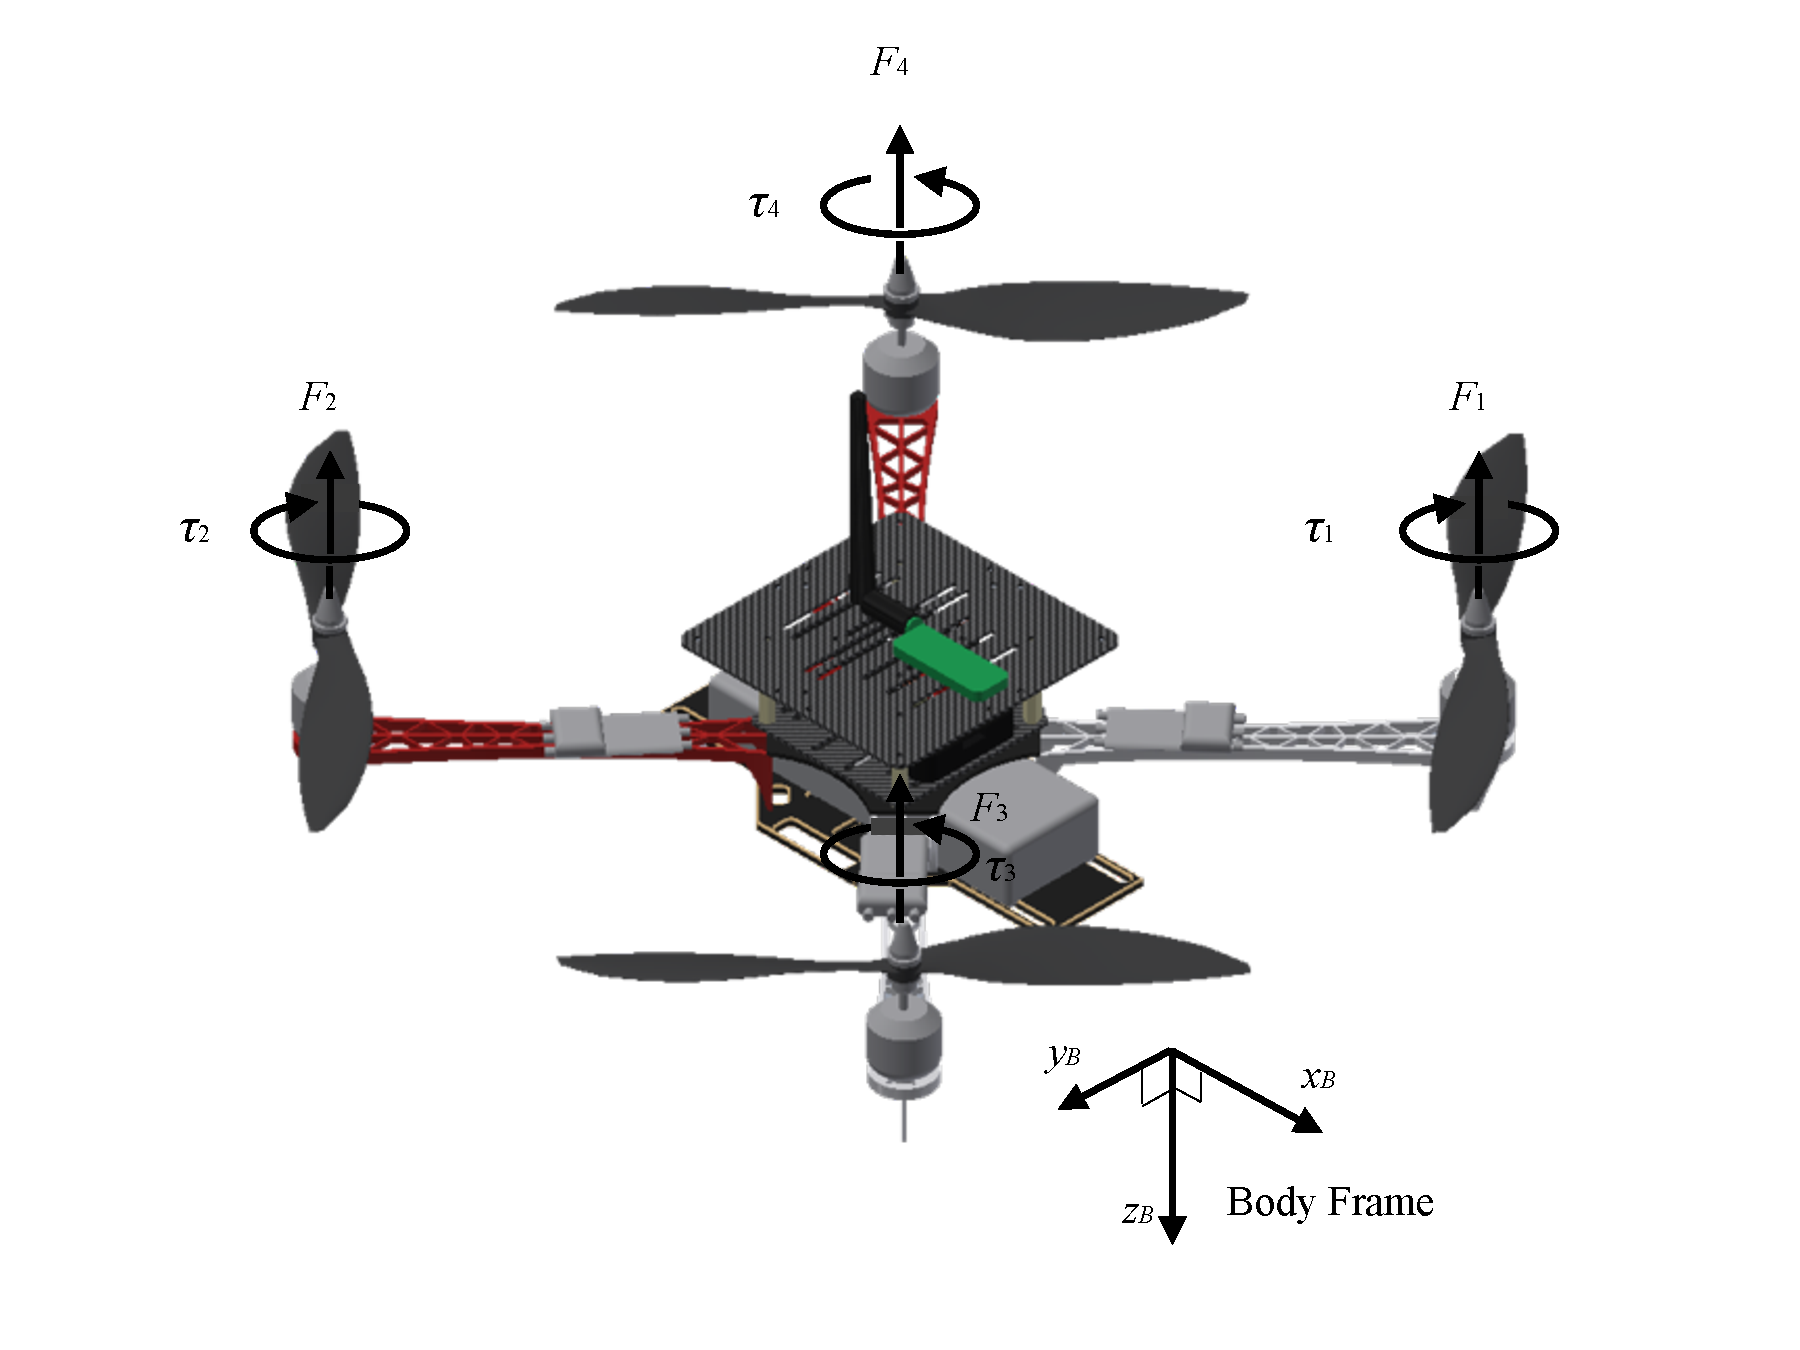
\includegraphics[width=0.8\textwidth]{graphics/mixer.pdf}
    \caption{Thrust and Torque Generated by Each Rotor}
    \label{fig:mixer}
\end{figure}

In the mixer, the magnitude of the desired thrust \(F_d\) from the outer-loop and the desired attitude control \({\boldsymbol \tau} = (\tau_{\phi}, \tau_{\theta}, \tau_{\psi})\) from the inner-loop are received. In order to map the attitude control and the desired thrust into motor speed \( {\boldsymbol n} = (n_1, n_2, n_3, n_4)\) , an aerodynamic model of the quadrotor can be applied.

It is known that the property of propeller is given with non-dimensional thrust coefficient \(C_T\) and power coefficient \(C_P\) as, \\
\begin{equation}
\begin{aligned}
C_T (n_i) ={ T \over { \rho {n_i}^2 D^4}}
\end{aligned}
\end{equation}
\begin{equation}
\begin{aligned}
C_P (n_i) = {P \over { \rho {n_i}^3 D^5}}
\end{aligned}
\end{equation}
where \(\rho\) is the density of air, \(D\) is the propeller's diameter, and \(T\), \(P\) are thrust and torque generated by a propeller, respectively \cite{airfoil2}. Here, \(C_T\) and \(C_P\) change according to rotation speed, and their curves are varied across different geometry of propellers and other conditions. Let \(F_i \) be the thrust force of each motor (\( i = 1, 2, 3, 4 \)) corresponding to its motor speed \( n_i\). With the experimental data of \(C_T\) and \(C_P\), thrust \( F_i\) and torque \(\tau_i\) generated by a motor according to its motor speed \( n_i\) are given as below,\\
\begin{equation}
\begin{aligned}
F_i = C_T (n_i) \rho {n_i}^2 D^4
\end{aligned}
\end{equation}
\begin{equation}
\begin{aligned}
\tau_i & = {P \over {2 \pi n_i}} \\ 
& = {C_P (n_i) \rho {n_i}^2 D^5 \over {2 \pi}}
\end{aligned}
\end{equation}

Since the quadrotor uses an X-shape frame in which the formation of the motors is a square, there is a linear relation as, \\
\begin{equation}
\begin{aligned}
F & = F_1 + F_2 + F_3 + F_4 \\
\tau_{\phi} & = {l \over {\sqrt{2}}} ( - F_1 + F_2 + F_3 - F_4)\\
\tau_{\theta} & = { l \over {\sqrt{2}}} (  F_1 - F_2 + F_3 - F_4)\\
\tau_{\psi} & =  \tau_1 + \tau_2 - \tau_3 - \tau_4
\end{aligned}
\end{equation}
where \(l\) to the length of the frame \cite{randal08}. We define an aerodynamic coefficient matrix \(B ({\boldsymbol n})\) as,
\begin{equation}
\begin{aligned}
B ({\boldsymbol n}) = 
\begin{bmatrix}
C_T (n_1)	& C_T (n_2)	& C_T (n_3)	& C_T (n_4)\\
- {l \over{\sqrt{2}}} C_T (n_1)		& {l \over{\sqrt{2}}} C_T (n_2)		& {l \over{\sqrt{2}}} C_T (n_3)	& - {l \over{\sqrt{2}}} C_T (n_4) \\
{l \over{\sqrt{2}}} C_T (n_1)		& - {l \over{\sqrt{2}}} C_T (n_2)		& {l \over{\sqrt{2}}} C_T (n_3)	& - {l \over{\sqrt{2}}} C_T (n_4) \\
{D \over{2\pi}} C_P (n_1)			& {D \over{2\pi}} C_P	 (n_2)		& - {D \over{2\pi}} C_P (n_3)	& - {D \over{2\pi}} C_P (n_4)
\end{bmatrix}
\end{aligned}
\end{equation}
Then, the above equation can be written as,\\
\begin{equation}
\label{eq:u_n}
\begin{aligned}
\begin{bmatrix}
F_d\\
u_p\\
u_q\\
u_r
\end{bmatrix}
= \rho D^4 B ({\boldsymbol n})
\begin{bmatrix}
{n_1}^2 \\
{n_2}^2 \\
{n_3}^2 \\
{n_4}^2
\end{bmatrix}
\end{aligned}
\end{equation}
With the above equation, motor speed \({\boldsymbol n} \) corresponding to the magnitude of the desired thrust \(F_d\) and the attitude control \({\boldsymbol \tau}\) can be computed as, \\
\begin{equation}
\label{eq:n_u}
\begin{aligned}
\begin{bmatrix}
{n_1}^2 \\
{n_2}^2 \\
{n_3}^2 \\
{n_4}^2
\end{bmatrix}
= {1 \over \rho D^4 }B^{-1} ({\boldsymbol n})
\begin{bmatrix}
F_d\\
u_p\\
u_q\\
u_r
\end{bmatrix}
\end{aligned}
\end{equation}


%%%%%%%%%%%%%%%%%%%%%%%%%%%%%%%%%%%%%%%%%%%%%%%%%%%%%%%%%%%%%%%%%%%%%%%%%%%%%%%%%%%%%%%%%%%%%%
\subsection{Approximation of the Aerodynamic Coefficient Matrix}
Since the coefficient matrix \( B ({\boldsymbol n}) \) is not independent from motor speed \(n_i\), it is difficult to compute a solution of Equation (\ref{eq:n_u}). To solve the problem, the linear approximation in terms of \(1 \over {n_i}^2\) as,\\
\begin{equation}
\label{eq:ct_approx}
\begin{aligned}
C_T ({n_i}) & = {C_T}_0 + {C_T}_1 {1 \over {n_i}^2} + O \left({1 \over {n_i}^4} \right) \\
& \approx {C_T}_0 + {C_T}_1 {1 \over {n_i}^2} \\
\end{aligned}
\end{equation}
\begin{equation}
\label{eq:cp_approx}
\begin{aligned}
C_P ({n_i}) & = {C_P}_0 + {C_P}_1 {1 \over {n_i}^2} + O \left({1 \over {n_i}^4} \right) \\
& \approx {C_P}_0 + {C_P}_1 {1 \over {n_i}^2}
\end{aligned}
\end{equation}
can be applied. Then, Equation (\ref{eq:u_n}) can be written as, \\
\begin{equation}
\begin{aligned}
\begin{bmatrix}
F_d\\
u_p\\
u_q\\
u_r
\end{bmatrix}
\approx \rho D^4 \left( B_0
\begin{bmatrix}
{n_1}^2 \\
{n_2}^2 \\
{n_3}^2 \\
{n_4}^2
\end{bmatrix}
+ B_1 
\begin{bmatrix}
1\\
1\\
1\\
1
\end{bmatrix} \right)
\end{aligned}
\end{equation}
where the approximation terms of \( B_0\), \(B_1\) of the matrix \(B ({\boldsymbol n}) \) are defined as,
\begin{equation}
\begin{aligned}
B_0 = 
\begin{bmatrix}
{C_T}_0	& {C_T}_0 	& {C_T}_0		& {C_T}_0 \\
- {l \over{\sqrt{2}}} {C_T}_0		& {l \over{\sqrt{2}}} {C_T}_0		& {l \over{\sqrt{2}}} {C_T}_0	& - {l \over{\sqrt{2}}} {C_T}_0 \\
{l \over{\sqrt{2}}} {C_T}_0		& - {l \over{\sqrt{2}}} {C_T}_0		& {l \over{\sqrt{2}}} {C_T}_0	& - {l \over{\sqrt{2}}} {C_T}_0 \\
{D \over{2\pi}} {C_P}_0			& {D \over{2\pi}} {C_P}_0		& - {D \over{2\pi}} {C_P}_0		& - {D \over{2\pi}} {C_P}_0
\end{bmatrix}
\end{aligned}
\end{equation}
\begin{equation}
\begin{aligned}
B_1 = 
\begin{bmatrix}
{C_T}_1	& {C_T}_1 	& {C_T}_1		& {C_T}_1 \\
- {l \over{\sqrt{2}}} {C_T}_1		& {l \over{\sqrt{2}}} {C_T}_1		& {l \over{\sqrt{2}}} {C_T}_1	& - {l \over{\sqrt{2}}} {C_T}_1 \\
{l \over{\sqrt{2}}} {C_T}_1		& - {l \over{\sqrt{2}}} {C_T}_1		& {l \over{\sqrt{2}}} {C_T}_1	& - {l \over{\sqrt{2}}} {C_T}_1 \\
{D \over{2\pi}} {C_P}_1			& {D \over{2\pi}} {C_P}_1		& - {D \over{2\pi}} {C_P}_1	& - {D \over{2\pi}} {C_P}_1
\end{bmatrix}
\end{aligned}
\end{equation}
Then, desired motor speeds \( \boldsymbol n\) are easily computed from the below equation,
\begin{equation}
\begin{aligned}
\begin{bmatrix}
{n_1}^2 \\
{n_2}^2 \\
{n_3}^2 \\
{n_4}^2
\end{bmatrix}
\approx
{B_0}^{-1}
\left(
{1 \over {\rho D^4}}
\begin{bmatrix}
F_d\\
u_p\\
u_q\\
u_r
\end{bmatrix}
- B_1
\begin{bmatrix}
1\\
1\\
1\\
1
\end{bmatrix}
\right)
\end{aligned}
\end{equation}

\begin{figure}
    \centering
    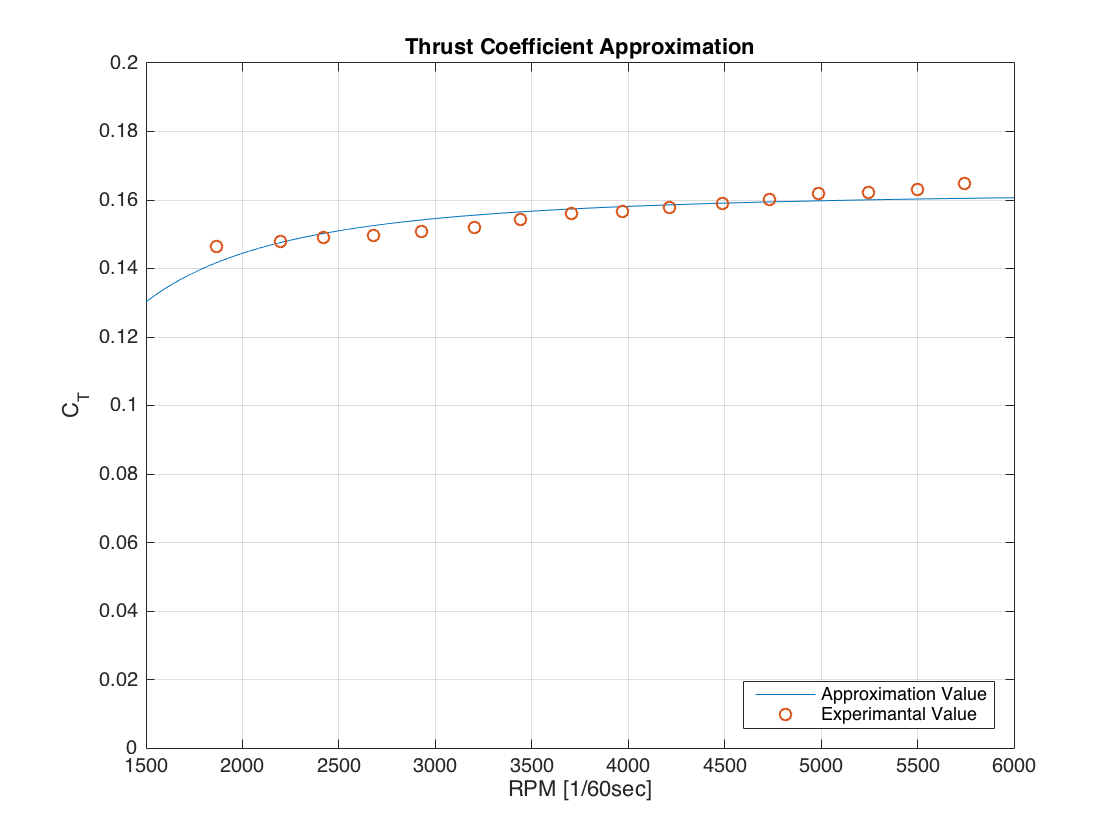
\includegraphics[width=0.8\textwidth]{graphics/Ct_fig.png}
    \caption{Comparison of experimental and approximated thrust coefficient}
    \label{fig:ct}
    
    \vspace{1cm}
    
    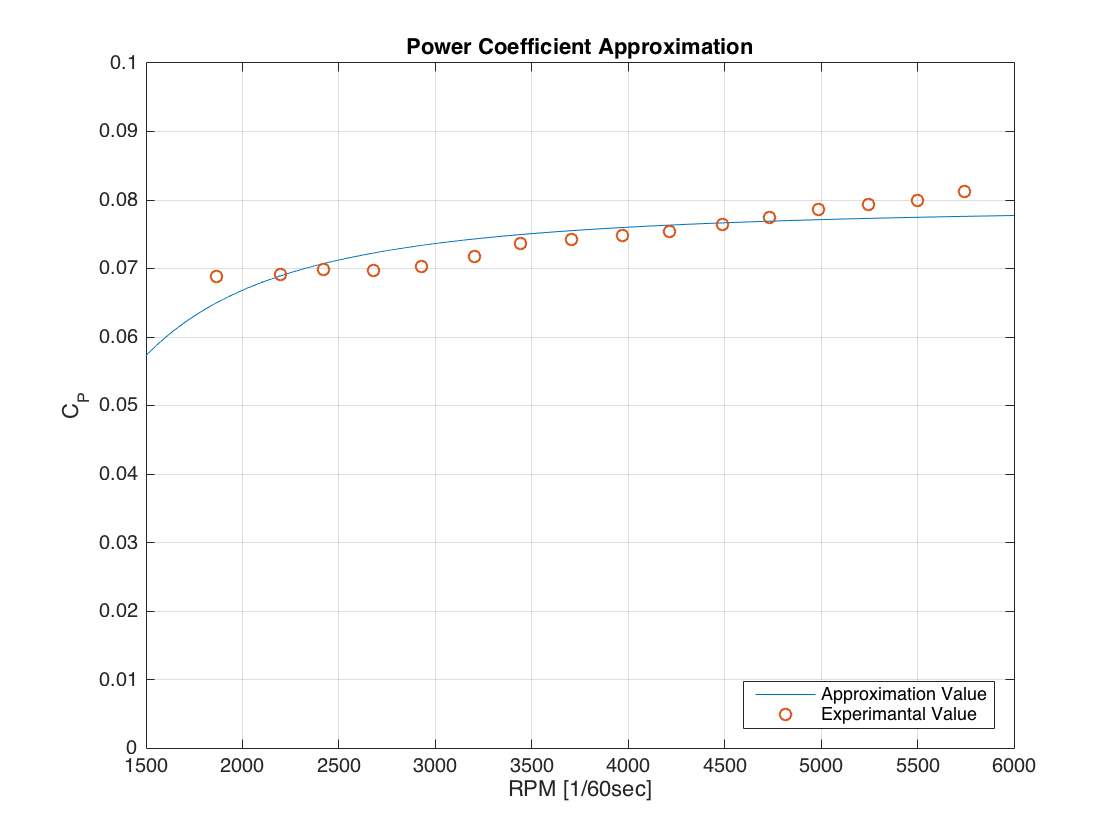
\includegraphics[width=0.8\textwidth]{graphics/Cp_fig.png}
    \caption{Comparison of experimental and approximated power coefficient}
    \label{fig:cp}
\end{figure}

To compute the model of thrust coefficient (\ref{eq:ct_approx}) and power coefficient (\ref{eq:cp_approx}), the experimental data of the propeller APC 10 \(\times\) 4.7 in the UIUC Propeller Database Vol.1 are used, and the method of least mean square error (LMSE) linear regression is applied in terms of \(1 \over {{n_i}^2}\) \cite{airfoil}. The approximated models of \(C_T (n_i)\) and \(C_P (n_i)\) are given as Equations (\ref{eq:ct}) and (\ref{eq:cp}), and the experimental data and the approximated models are compared in the Figures \ref{fig:ct}, \ref{fig:cp}. \\
\begin{equation}
\label{eq:ct}
\begin{aligned}
C_T ({n_i}) & = 0.1627 -73047 \times {1 \over {n_i}^2} \\
\end{aligned}
\end{equation}
\begin{equation}
\label{eq:cp}
\begin{aligned}
C_P ({n_i}) & = 0.0791 - 49112 \times {1 \over {n_i}^2} \\
\end{aligned}
\end{equation}
%%%%%%%%%%%%%%%%%%%%%%%%%%%%%%%%%%%%%%%%%%%%%%%%%%%%%%%%%%%%%%%%%%%%%%%%%%%%%%%%%%%%%%%%%%%%%%
\subsection{Motor Control}
In the quadrotor system, propellers are rotated by four brushless DC motors. In order to control DC motors, the method of pulse width modulation (PWM) is often used. In the PWM method, an average of constant-voltage pulsing signals actuates a motor \cite{audio}. Therefore, motor voltage is controllable by changing a pulse signal's width. Let \(d_{pwm}\) be duty cycle as, \\
\begin{equation}
\begin{aligned}
d_{pwm} = H f_{pwm} : \quad 0 \le d_{pwm} \le 1
\end{aligned}
\end{equation}
where \(H\) is signal width and \(f_{pwm}\) is the fixed frequency of signals. Then, the relation between motor voltage \(V_{mot}\) and duty cycle \(pwm\) is formalized as, \\
\begin{equation}
\label{eq:pwm_voltage}
\begin{aligned}
V_{mot} = d_{pwm} V_0
\end{aligned}
\end{equation}
where \(V_0\) is the constant voltage of signals.

The electric and dynamic models of a DC motor are given in terms of motor speed \(n\) and \(V_{mot}\) as,
\begin{equation}
\label{eq:motor_dynamics_01}
\begin{aligned}
V_{mot} & = 2 \pi k_{b} n + R i + L {{di}\over {dt}}\\
\end{aligned}
\end{equation}
\begin{equation}
\label{eq:motor_dynamics_02}
\begin{aligned}
k_m i & = 2 \pi k_f n + 2 \pi I_{mot} {{dn} \over {dt} } + M_R \text{sgn} (n)
\end{aligned}
\end{equation}
{\color{blue} where \(k_{b} \), \(k_f\), \(k_m\) are the motor's back electromotive force constant, viscous damping coefficient, and torque constant, respectively.} \(M_R\) is frictional torque, \(R\) is the motor's internal resistor, and \(L\) is the motor's internal inductance \cite{Mahfouz13}. \(I_{mot}\) is the total inertia of the motor and the propeller. Then, the above equation is written as the following second-order system with respect to motor speed \(n\). \\
\begin{equation}
\label{eq:motor_model_01}
\begin{aligned}
V_{mot} = 2 \pi \left( (k_b + {{R k_f}\over{k_m}} ) n + {1 \over {k_m}}( {R I_{mot}} + L k_f ) {{dn}\over{dt}} + {{L I_{mot}} \over {k_m} } {{d^2 n}\over{{dt}^2}}  \right) + R M_R \text{sgn} (n) : \quad n \neq 0\\
\end{aligned}
\end{equation}
Also, from Equation (\ref{eq:motor_dynamics_02}), there is a voltage threshold due to frictional torque so that a motor doesn't spin below the threshold. \\

Assuming motor speed changes smoothly so that the effect of internal resistor and inductance is small enough, Equation (\ref{eq:motor_model_01}) can be simplified as, \\
\begin{equation}
\label{eq:motor_model_02}
\begin{aligned}
V_{mot} \approx 2 \pi  (k_b + {{R k_f}\over{k_m}} ) n  + R M_R \text{sgn} (n)
\end{aligned}
\end{equation}
Define composite coefficients of the tangent \(\alpha\), and the intercept \(\beta\) as, 
\begin{equation}
\begin{aligned}
\alpha = {{k_m V_0} \over {2 \pi (k_b k_m + R k_f )}} 
\end{aligned}
\end{equation}
\begin{equation}
\begin{aligned}
\beta = {{k_m R M_R} \over {2 \pi (k_b k_m + R k_f )}} 
\end{aligned}
\end{equation}
Then, from Equations (\ref{eq:pwm_voltage}) and (\ref{eq:motor_model_02}), the relation between the motor speed \(n\) and the duty cycle \(d_{pwm}\) is written as the below equation.  \\
\begin{equation}
\label{eq:motor_curve_01}
\begin{aligned}
n \approx 
\begin{cases}
     \alpha d_{pwm}  - \beta \quad &  d_{threshold} \le d_{pwm} \le 1 \\
    0  \quad &   d_{pwm} \le  d_{threshold} \\
  \end{cases}
  \end{aligned}
\end{equation}

\begin{figure}
    \centering
    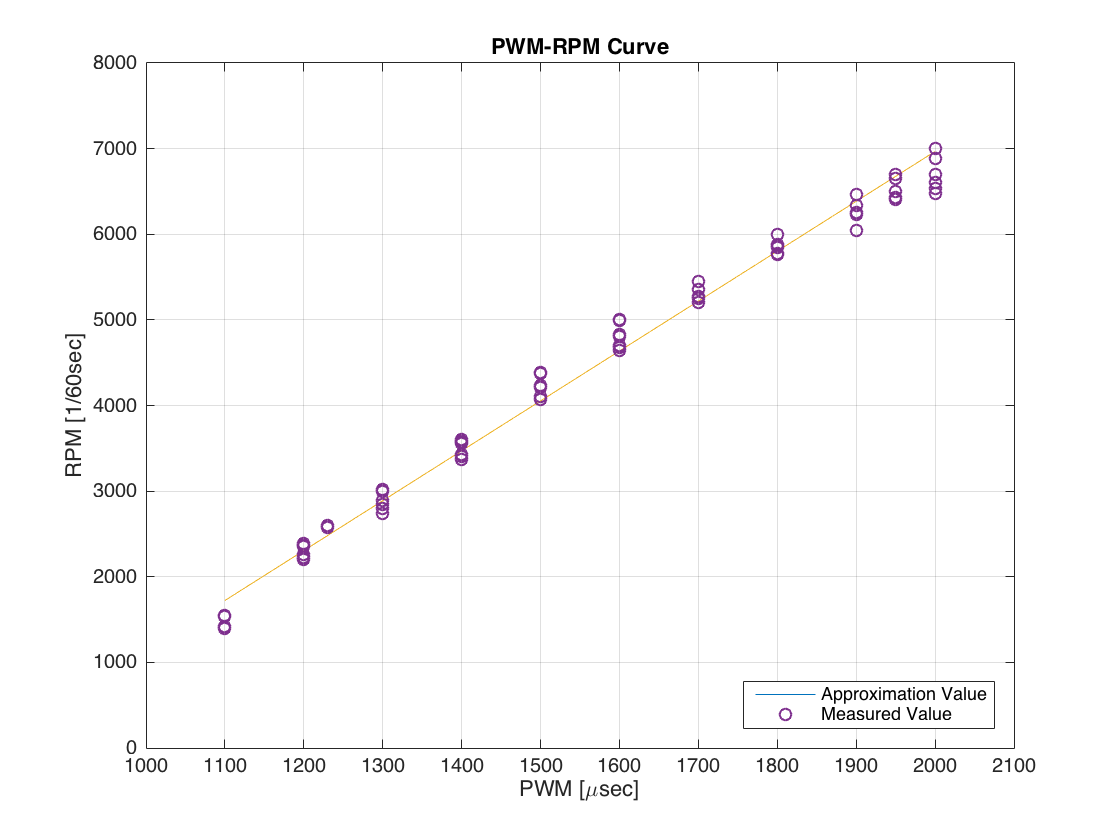
\includegraphics[width=0.8\textwidth]{graphics/pwm_rpm_curve.png}
    \caption{Change of RPM output corresponding to PWM command}
    \label{fig:pwm_rpm}
\end{figure}
If the characteristic information of the motors is available, the parameters \(\alpha\), \(\beta\) of the model of Equation (\ref{eq:motor_curve_01}) can be computed. However, there is no available information about the motor constants, it is necessary to calibrate the relation between PWM input and RPM output of a motor with a propeller. Therefore, the composite parameters of the gradient \(\alpha\) and the intercept \(\beta\) are calibrated by experiments. In the calibration, a reflective marker sticker is put on each propeller, and a tachometer measures rotation speed of the markers. PWM signal of voltage is controlled by an ESC, and the range of PWM command is set to be between 1000 \(\mu\)sec and 2000 \(\mu\)sec. The result of the experiment and the approximated model by the LMSE linear regression method are shown in Figure \ref{fig:pwm_rpm} and Equation (\ref{eq:motor_curve_02}).\\
\begin{equation}
\label{eq:motor_curve_02}
\begin{aligned}
n = 
\begin{cases}
     0.1716 \times d_{pwm}  - 803.4 \quad &  1100 \le d_{pwm} \le 2000 \\
    0  \quad &   \text{otherwise} \\
  \end{cases}
  \end{aligned}
\end{equation}


Since a brushless DC motor used in the quadrotor system does not have an encoder to measure its motor speed, open-loop control based on Equation (\ref{eq:motor_curve_02}) is applied to control motor speed. Also, PWM command is limited to be between 1230 \(\mu\)sec and 1950 \(\mu\)sec to prevent inappropriate performance.
